\documentclass[10pt]{beamer}

%\usepackage[backend=bibtex,firstinits=true,style=verbose-inote,citestyle=authortitle]{biblatex}
\usepackage{bm}
\usepackage{graphicx}
\usepackage{subcaption}
\usepackage{amsmath}
\usepackage{amsfonts}
\usepackage{makecell}
\usepackage{filecontents}
\usepackage{biblatex}
%\usepackage[english]{babel}
\usepackage[utf8]{inputenc}
\usepackage{fancyhdr}
\usepackage{amsmath,amssymb,amsfonts,amsthm}
\usepackage{indentfirst}
\usepackage{bm}
\usepackage[a4paper, total={6in, 10in}]{geometry}

% For using subfigures
\usepackage{graphicx}
\usepackage{caption}
\usepackage{subcaption}

% To put a figure where it is
\usepackage{float}

\usepackage{tensor}
\usepackage{biblatex}
\usepackage{titlesec}
\usepackage{bbm, dsfont} % For indicator functions
\usepackage{mathtools} % for \coloneqq
\usepackage[bottom]{footmisc} % prevents pictures going below footnote :|
% \usepackage{pifont} % for \ding{...}

\addbibresource{../../articles/articles.bib}

% \newcommand\defeq{\stackrel{\mathclap{\normalfont\mbox{def}}}{=}}

\newcommand{\expect}[2][]{
\ifthenelse{\equal{#1}{}}{
\mathbb{E}\left[#2\right]
}{
\underset{#1}{\mathbb{E}}\left[#2\right]
}}

\newcommand{\cov}[2][]{
\ifthenelse{\equal{#1}{}}{
\text{Cov}\left[#2\right]
}{
\underset{#1}{\text{Cov}}\left[#2\right]
}}


\newcommand{\var}[2][]{
\ifthenelse{\equal{#1}{}}{
\text{Var}[#2]
}{
\underset{#1}{\text{Var}}[#2]
}}

\newcommand{\loss}[2][]{
\ifthenelse{\equal{#1}{}}{
\mathcal{L}(#2)
}{
\mathcal{L}_{#1}(#2)
}}

\newcommand{\kl}[2]{
\text{D}_\text{KL}[#1 \parallel #2]
}

\newcommand{\R}{\mathbb{R}}
%\newcommand{\Prob}{\mathbb{P}}

\newcommand{\1}[1]{\mathds{1}\{#1\}}

% We need this for \begin{theorem}...\end{theorem} staff
\newtheorem*{theorem*}{Theorem}
\newtheorem{theorem}{Theorem}
\newtheorem*{proposition*}{Proposition}
\newtheorem{proposition}{Proposition}
\newtheorem*{corollary*}{Corollary}
\newtheorem{corollary}{Corollary}
\newtheorem*{lemma*}{Lemma}
\newtheorem{lemma}{Lemma}
\newtheorem*{question*}{Question}
\newtheorem{question}{Question}

\theoremstyle{definition}
\newtheorem{definition}{Definition}[section]


\newcommand{\expect}[2][]{
\ifthenelse{\equal{#1}{}}{
\mathbb{E}\left[#2\right]
}{
\underset{#1}{\mathbb{E}}\left[#2\right]
}}

%\usecolortheme{dolphin}
\setbeamertemplate{navigation symbols}{}
\setbeamertemplate{section in toc}{\inserttocsectionnumber.~\inserttocsection}

\begin{filecontents*}{references.bib}
@inproceedings{
GAN_steerability,
title={On the "steerability" of generative adversarial networks},
author={Ali Jahanian* and Lucy Chai* and Phillip Isola},
booktitle={International Conference on Learning Representations},
year={2020},
url={https://openreview.net/forum?id=HylsTT4FvB}
}
\end{filecontents*}

\addbibresource{references.bib}


\title{On the "steerability" of generative adversarial networks\footnote{\citepaper{GAN_steerability}}}
%\subtitle{}
%\author{Ivan Skorokhodov}
%\date{}
%\logo{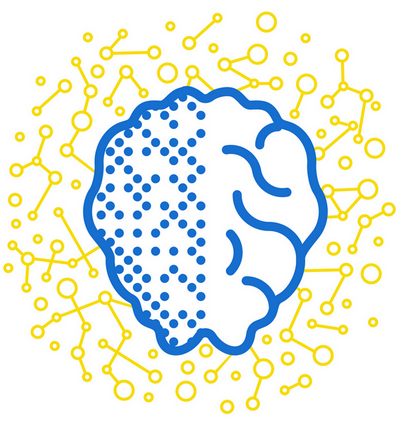
\includegraphics[height=1cm]{images/ipavlov-logo.png}}

\newcommand{\citepaper}[1]{\citetitle{#1} by \citeauthor{#1}}

%\graphicspath{{./images}}

%\usetheme{lucid}
\begin{document}

\begin{frame}
    \titlepage
\end{frame}

\begin{frame}{What this paper is about?}
    \begin{itemize}
        \item\pause It is believed that neural networks do not generalize ``outside'' of a dataset
        \item\pause Do GANs suffer from the same issue?
        \item\pause Yes :(
        \item\pause But we can zoom/rotate/shift generated images by simple manipulations in latent space
\begin{figure}
    \centering
    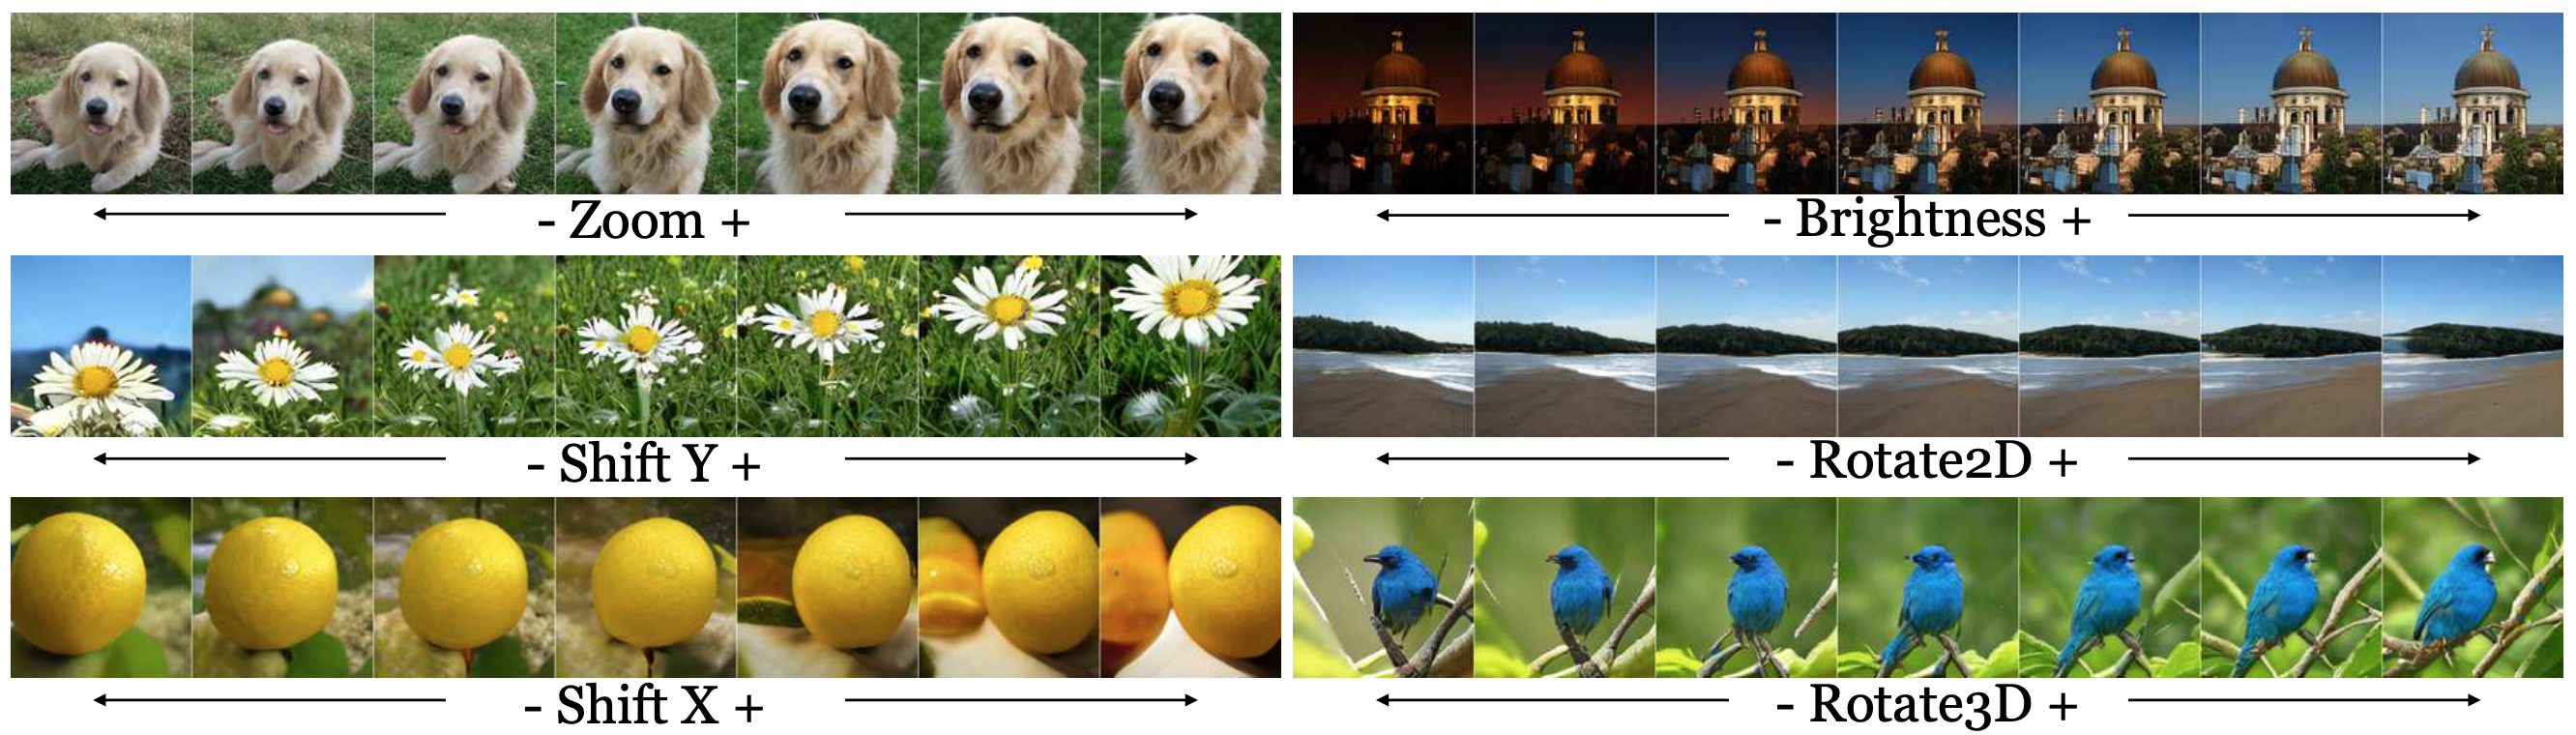
\includegraphics[width=\textwidth]{images/gan-steerability-examples.png}
\end{figure}
        \item\pause We can also add an additional loss term to improve \textit{steerability}
        \item\pause This all shows us that GANs have some extrapolation abilities (but not a lot)
    \end{itemize}    
\end{frame}

\begin{frame}{What is steerability?}
    \pause
    GAN model is \textit{steerable} if we can change a specific property of an image by ``walking'' in a latent space.
    
    \begin{figure}
        \centering
        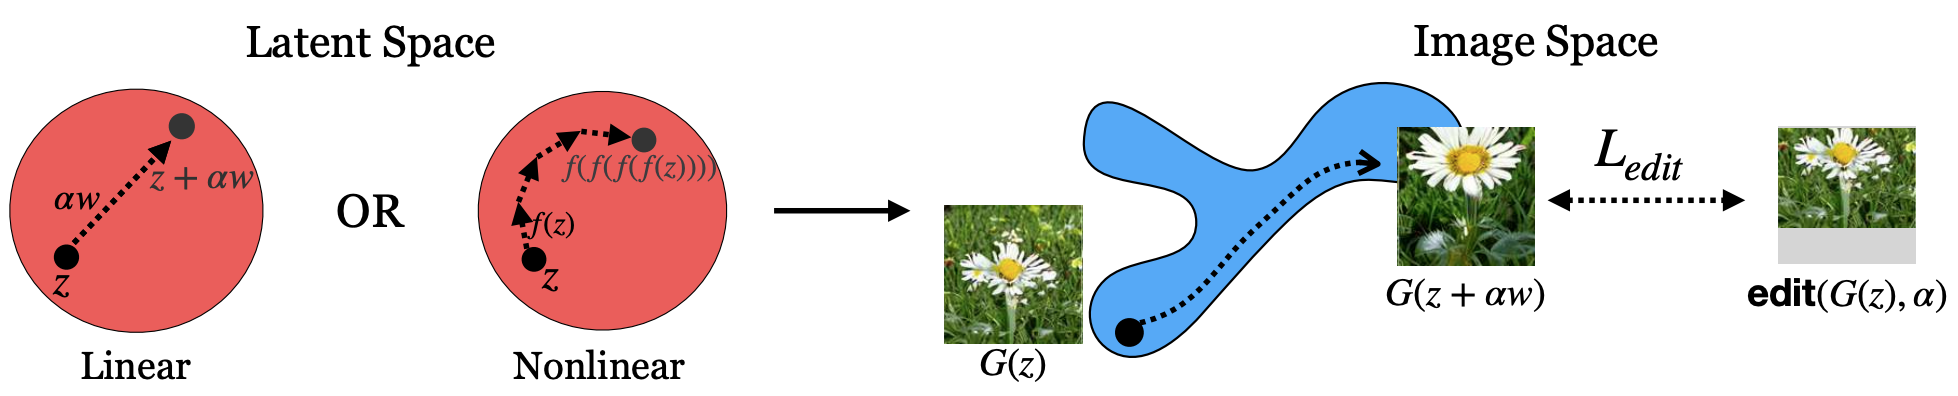
\includegraphics[width=\textwidth]{images/gan-steerability-walking-example.png}
    \end{figure}
    
    On the image above:
    \begin{itemize}
        \item\pause We move via a linear or a nonlinear path in the latent space
        \item\pause The daisy image shifts up in the image space
        \item\pause (We can also construct a supervised signal by cropping and shifting the image, like in the rightmost image)
    \end{itemize}
\end{frame}

\begin{frame}{How to construct a path in a latent space?}
    How do we build a linear path in a latent space?
    
    \begin{enumerate}
        \item\pause Imagine that we want to find a path for zooming
        \item\pause Generate a lot of synthetic images
        \item\pause Edit these synthetic images by zooming-in and zooming-out with different strengths
        \item\pause Find optimal path direction $w$ by optimizing\footnote{Instead of using L2 loss one can use perceptual distance, but this does not change things much}:
        \begin{equation}
w^{*}=\underset{w}{\arg \min } \expect[z, \alpha]{\| G(z+\alpha w) - \operatorname{edit}(G(z), \alpha) \|_2^2}
\end{equation}
    \end{enumerate}
    Here:
    \begin{itemize}
        \item $\operatorname{edit}(G(z), \alpha)$ is the edited image
        \item $\alpha$ is a strength parameter
    \end{itemize}
\end{frame}

\begin{frame}{How to construct a path in a latent space?}
How do we build a non-linear path in a latent space?

\begin{enumerate}
    \item\pause We split a path into $n$ pieces of size $\epsilon$
    \item\pause We want to find a function $f_\theta$ such that applying it $n$ times will zoom an image in $n \cdot \epsilon$ times
    \item\pause We find it by optimizing:
    \begin{equation*}
        \theta^* = \arg\min_\theta \expect[z, n]{\| G(\underbrace{f(f(...f(}_{n\ \text{times}}z)))) - \operatorname{edit}(G(z), n\cdot\epsilon)\|_2^2}
    \end{equation*}
    Authors parametrize $f$ as a neural network.
\end{enumerate}

\pause
But it does not work much better than a linear path:
\begin{figure}
    \centering
    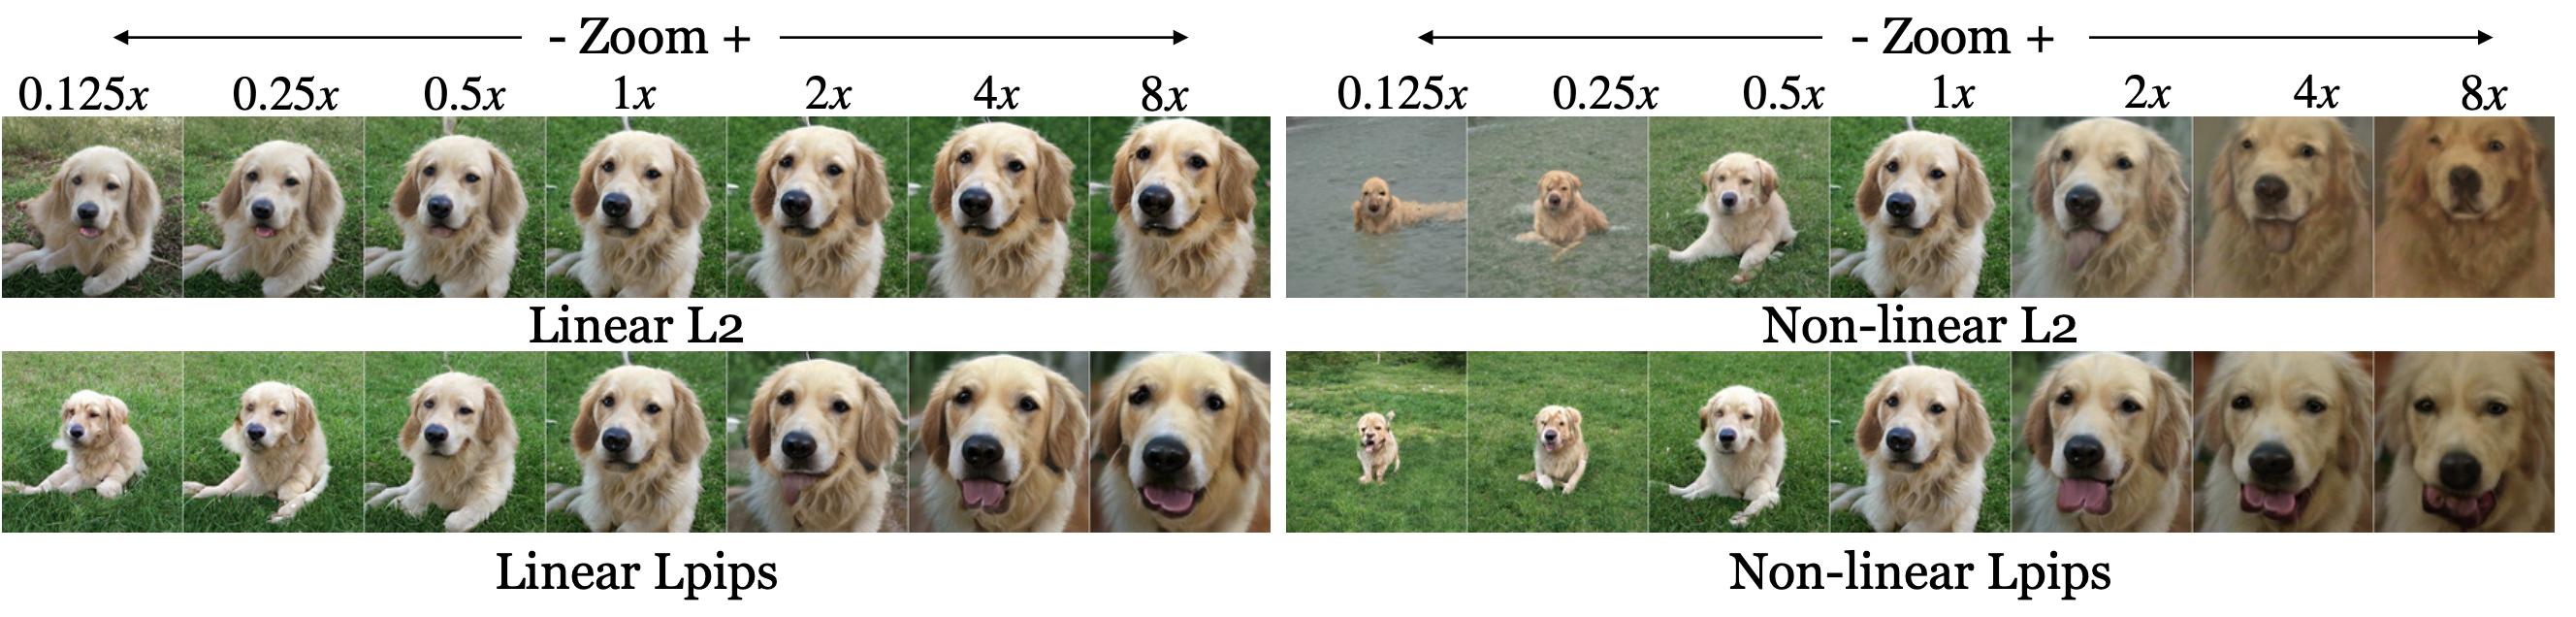
\includegraphics[width=\textwidth]{images/gan-steerability-linear-vs-nonlinear.png}
\end{figure}

\end{frame}


\begin{frame}{Can we improve steerability?}
\pause Yes, by adding an additional regularization to Generator's objective:

\begin{equation}
G^{*}, w^{*}=\arg \min_{G, w}\left(\mathcal{L}_{e d i t}+\mathcal{L}_{G A N}\right)
\end{equation}

Where:
\begin{equation}
\mathcal{L}_{e d i t}=L 2(G(z+\alpha w)-\operatorname{edit}(G(z), \alpha))
\end{equation}

And GAN loss is \footnote{Authors do not elaborate if $D$ is also trained with the modified loss}:
\begin{equation}
\mathcal{L}_{G A N}=\max _{D}\left(\mathbb{E}_{z, \alpha}[D(G(z+\alpha w))]-\mathbb{E}_{x, \alpha}[D(\operatorname{edit}(x, \alpha))]\right)
\end{equation}
\end{frame}


\begin{frame}{Steering has limits}
    There 2 types of problems we face when steer further:
    \begin{itemize}
        \item\pause Images become unrealistic
        \item\pause Images stop changing anymore
    \end{itemize}
    
    \begin{figure}
        \centering
        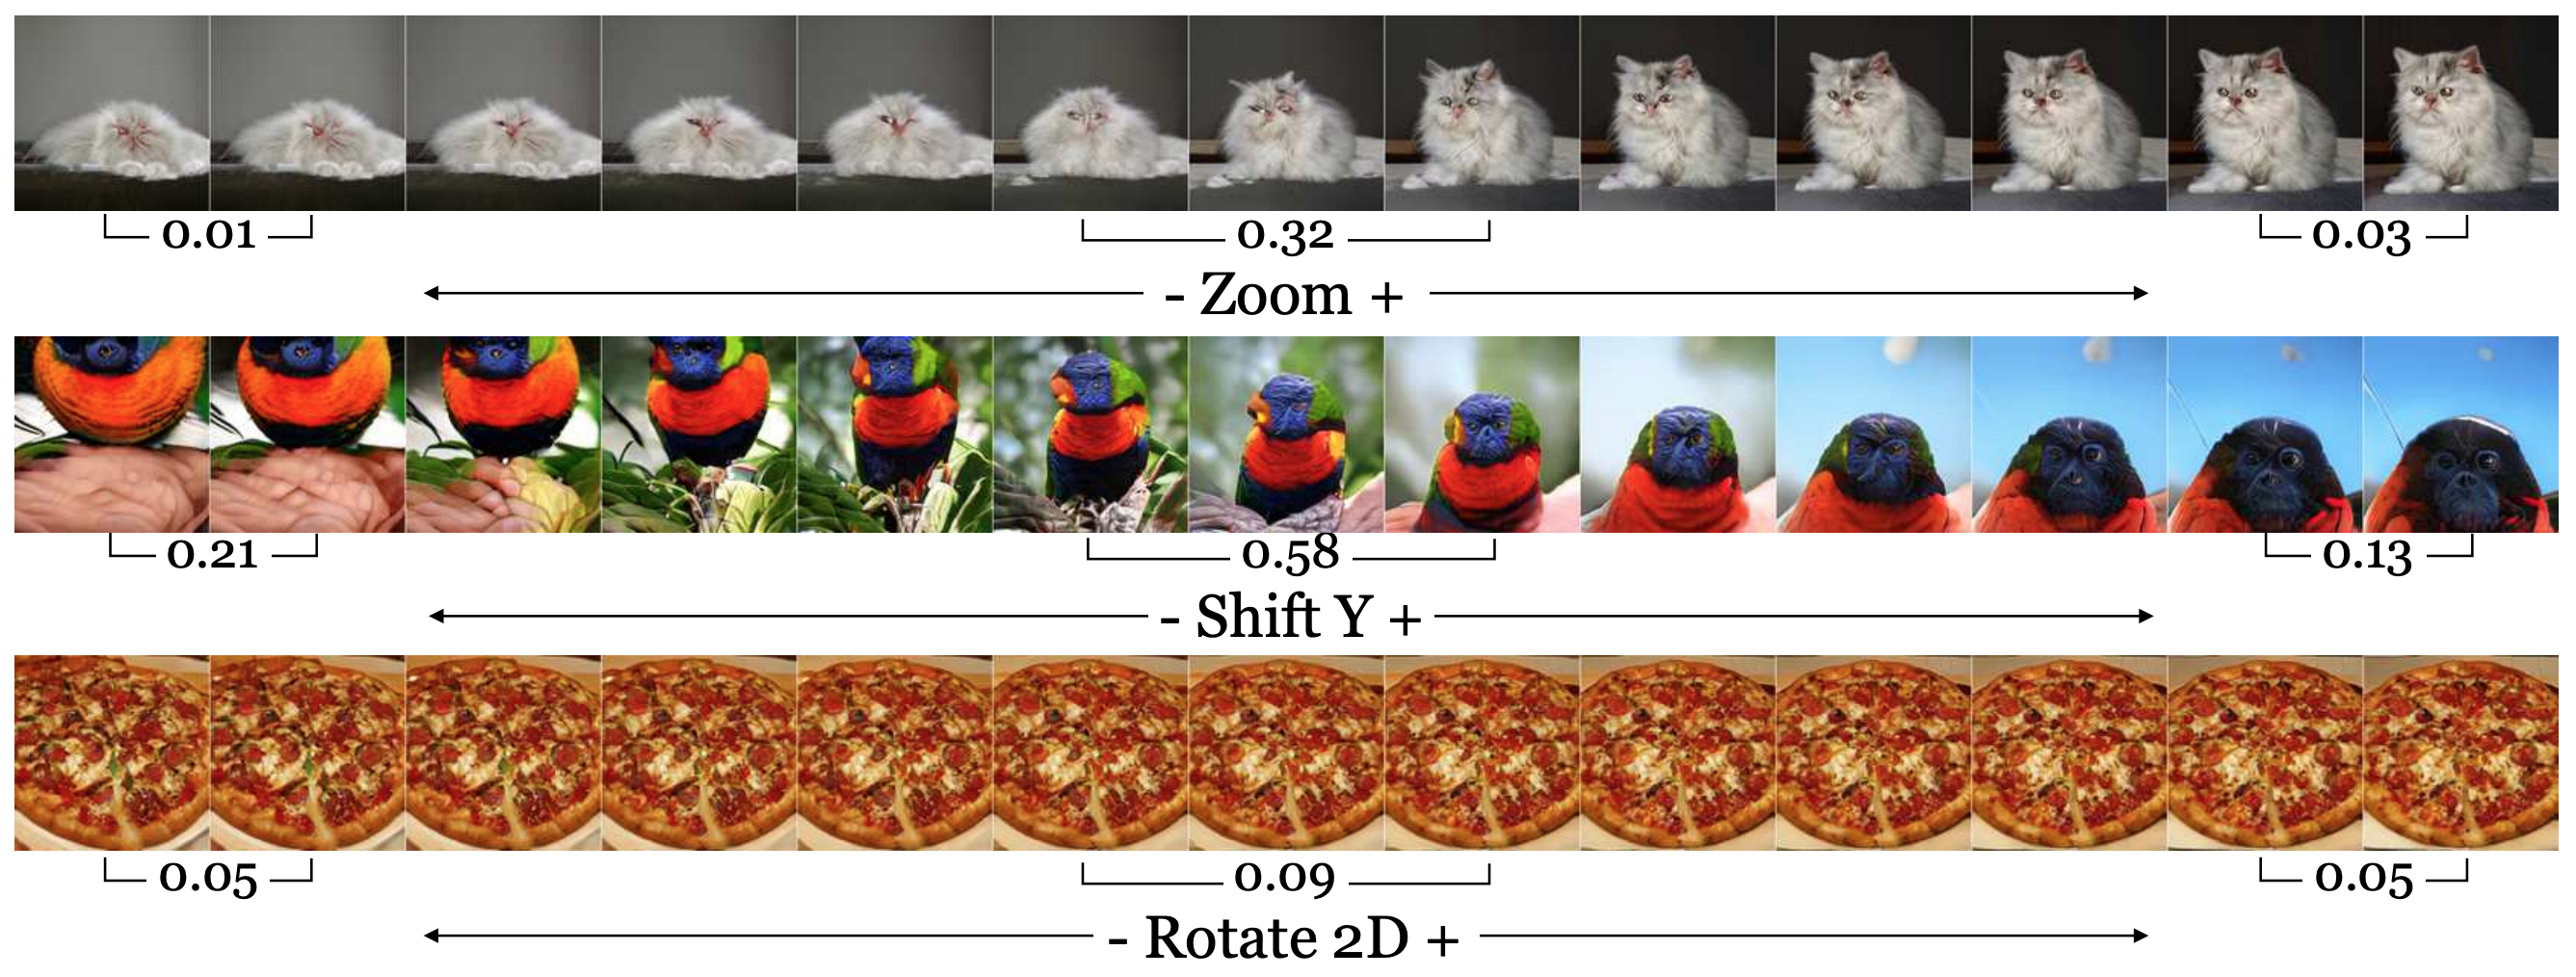
\includegraphics[width=\textwidth]{images/gan-steerability-failures.png}
    \end{figure}
    
    Numbers in the image are perceptual distances between images, showing that transformation converged.
\end{frame}

\begin{frame}{Conclusion}
    \begin{itemize}
        \item\pause Authors test steerability for several existing GAN models (BigGAN, StyleGAN, etc)
        \item\pause Authors proposed a way to quantify steerability (omitted in the presentation)
        \item\pause We need better editions for shifting/rotating/etc to find better paths
        \item\pause Variability in data allows us to build more steerable models
    \end{itemize}
\end{frame}

\end{document}
